\documentclass{article}

% \usepackage[paperwidth=190mm,paperheight=330mm, margin={.5in,.6in}]{geometry}
\usepackage[a4paper, margin={.5in,1in}]{geometry}
\usepackage{amsmath}
\usepackage{amssymb}
\usepackage{mathdots}
\usepackage{graphicx}
\usepackage{tikz}
\usetikzlibrary{arrows,matrix,positioning}
\usetikzlibrary{decorations.markings}
\usetikzlibrary{arrows.meta}
\usetikzlibrary{fit}
\usepackage{amsfonts}
\usepackage{amsthm}
\usepackage{pgfplots}
\pgfplotsset{compat=1.18}
\usepackage{extarrows}

\usepackage{cancel}

\theoremstyle{definition}
\newtheorem*{example}{Example}
\theoremstyle{definition}
\newtheorem*{answer}{Answer}

\newtheorem{theorem}{Theorem}[section]
\newtheorem{lemma}[theorem]{Lemma}

\theoremstyle{remark}
\newtheorem*{remark}{Remark}


\begin{document}
\title{Calculus Overview: Multivariable Differentiation}
\author{Foo}
\maketitle

\section{Concepts}

\newcommand{\jlm}[4]{\lim_{(#1, #2)\to(#3, #4)}}
\newcommand{\lmxy}[2]{\jlm{x}{y}{#1}{#2}}
\newcommand{\lmxyoo}{\lmxy{0}{0}}
\newcommand{\dd}{\textrm{d}}

\subsection{Multiple Limits}

Definition:
\[
    \lmxyoo f(x,y) = L
\]
if for every $\epsilon > 0$, there exists $\delta > 0$ such that when
\[
    0 < \sqrt{(x-x_0)^2 + (y-y_0)^2} < \delta,
\]
we have $|f(x,y) - L| < \epsilon$.

Usually, to prove that limits do not exist,
we choose different paths approaching $(x_0,y_0)$ 
and show that the limits along those paths are different.

\begin{theorem}
\label{thm:xayb_over_x2y2_lim}
For $\dfrac{x^{\alpha}y^{\beta}}{x^2+y^2}$ we use polar coordinates to
determine the limit as $r \to 0$. ($\alpha, \beta>0$)
\[
	\lmxyoo \frac{x^{\alpha}y^{\beta}}{x^2+y^2}
	= \lim_{r \to 0^{+}} 
	\frac{r^{\alpha+\beta} \cos^{\alpha} \theta \sin^{\beta} \theta }{r^2}
	= \lim_{r \to 0^{+}} r^{\alpha+\beta-2} \cos^{\alpha} \theta \sin^{\beta} \theta
	= \begin{cases}
		0 & \text{if } \alpha + \beta > 2 \\
		\text{does not exist} & \text{if } \alpha + \beta \leq 2
	\end{cases}
	\]
\end{theorem}

\begin{example}
	Also useful with similar form:
	\[
		\lmxyoo \frac{x^2y^2}{(x^2+y^2)^{\frac{3}{2}}}
		= \lmxyoo \left( \frac{x^{\frac{4}{3}}y^{\frac{4}{3}}}{x^2+y^2} \right)^{\frac{3}{2}}
		= 0
	\] 
\end{example}

\begin{example}
	By substituting variables, we can apply the same method to more cases.
	\[
		\lmxyoo \frac{x^{6}y^{7}}{x^{6}+y^{8}}
		\xlongequal[v=y^4]{u=x^3}
		\jlm{u}{v}{0}{0^{+}} \frac{u^2v^{\frac{7}{4}}}{u^2+v^2}
	=0
	\] 
\end{example}

But be careful that after converting to polar coordinates, \textbf{limits along
all fixed angles may exist without implying that the original limit exists.}

\begin{example}
	\[
		f(x, y) = \frac{x^2y}{x^4+y^2}
	\] 
In polar coordinates, we have
\[
	f(r, \theta) = \frac{r^2 \cos^2 \theta \sin \theta}{r^4 \cos^4 \theta + r^4 \sin^2 \theta}
	= \frac{r\cos^2 \theta \sin \theta}{r^2 \cos^4 \theta + \sin^2 \theta}
\]
For any fixed $\theta$, we have $\lim_{r \to 0} f(r, \theta) = 0$.
However, if we choose the path $y = x^2$, we have
\[
	\lim_{x \to 0} f(x, x^2) = \lim_{x \to 0} \frac{x^{4}}{2x^{4}} = \frac{1}{2}
\]

The key point is that when we approach $(0,0)$ along the path $y = x^2$, the
angle $\theta$ is not fixed, but approaches $0$ as $x \to 0$. Actually, we
cannot conclude that the limit $\lim_{(x,y) \to (0,0)} f(x,y)$ exists.
	
\end{example}

\subsection{Differentiability}

Definition:
$f$ is differentiable at $(x_0,y_0)$ if there exist $A$ and $B$ such that
\[
	\Delta f = A \Delta x + B \Delta y + o(\sqrt{(\Delta x)^2 + (\Delta y)^2})
\] 
Or equivalently, we can write
\[
	\jlm{\Delta x}{\Delta y}{0}{0}
	\frac{\Delta f - A \Delta x - B \Delta y}{\sqrt{(\Delta x)^2 + (\Delta y)^2}} = 0
\]

When $f$ is differentiable at $(x_0,y_0)$, we have

\[
\dd f = A \dd x + B \dd y = f_x(x_0,y_0) \dd x + f_y(x_0,y_0) \dd y
\] 

\begin{center}
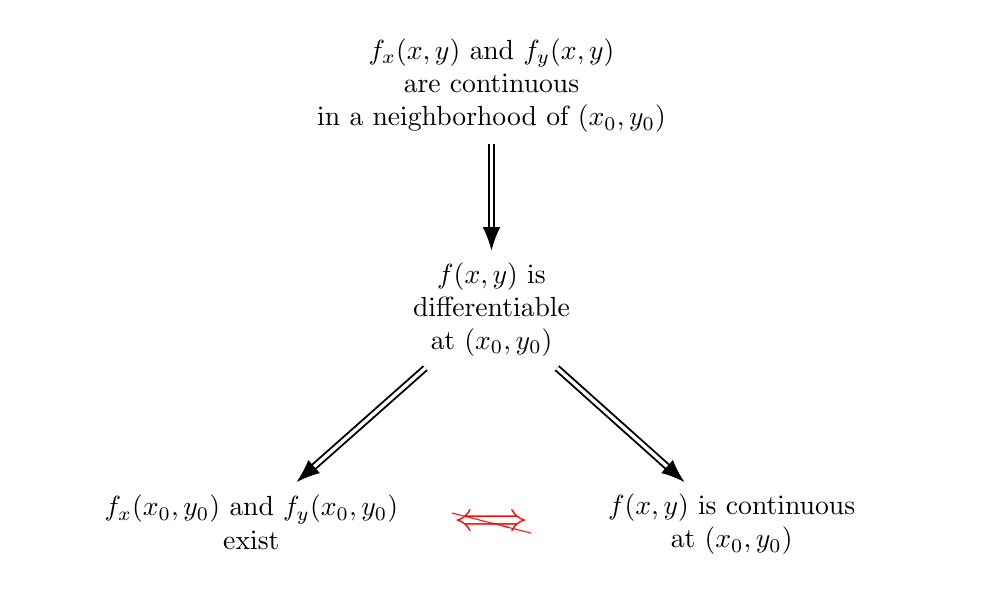
\begin{tikzpicture}[
    node distance=1.35cm,
    statement/.style={
        align=center,
        font=\normalsize,
        text width=5.4cm,
        minimum height=1cm,
        inner sep=4pt
    },
    implication/.style={
        -{Latex[length=3mm]},
        double,
        double distance=1.2pt,
        line width=0.7pt
    }
]

% Nodes
\node[statement] (continuous-partials)
{
    $f_x(x,y)$ and $f_y(x,y)$ are continuous\\
    in a neighborhood of $(x_0,y_0)$
};

\node[statement, below=of continuous-partials] (differentiable)
{
    $f(x,y)$ is\\
    differentiable\\
    at $(x_0,y_0)$
};

\node[statement, below=1.45cm of differentiable, xshift=-3.05cm] (partials-exist)
{
    $f_x(x_0,y_0)$ and $f_y(x_0,y_0)$\\
    exist
};

\node[statement, below=1.45cm of differentiable, xshift=3.05cm] (continuous)
{
    $f(x,y)$ is continuous\\
    at $(x_0,y_0)$
};

% Implications
\draw[implication] (continuous-partials) -- (differentiable);
\draw[implication] (differentiable) -- (partials-exist);
\draw[implication] (differentiable) -- (continuous);

\path (partials-exist.east) -- (continuous.west)
    node[midway, text=red, font=\Large] {$\bcancel\Longleftrightarrow$};

\end{tikzpicture}
\end{center}

\begin{theorem}
	If $f(x, y)$ is continuous at $(x_0, y_0)$ and
	 \[
		 \lmxy{x_0}{y_0} \frac{f(x,y) - Ax - By - C}{\sqrt{(x-x_0)^2 + (y-y_0)^2}} = 0
	\] 
	then $f$ is differentiable at $(x_0, y_0)$ and $A = f_x(x_0, y_0)$, $B = f_y(x_0, y_0)$.
	
\end{theorem}

\begin{proof}
Let
\[
r=\sqrt{(x-x_0)^2+(y-y_0)^2}.
\]
since \(r\to 0\) as \((x,y)\to (x_0,y_0)\), we have
\[
f(x,y)-Ax-By-C\to 0.
\]
using the continuity of \(f\) at \((x_0,y_0)\), it follows that
\[
f(x_0,y_0)-Ax_0-By_0-C=0.
\]
thus
\[
C=f(x_0,y_0)-Ax_0-By_0.
\]
therefore the assumed limit becomes
the definition of differentiability of \(f\) at \((x_0,y_0)\).
\[
\lim_{(x,y)\to (x_0,y_0)}
\frac{
f(x,y)-f(x_0,y_0)-A(x-x_0)-B(y-y_0)
}{
\sqrt{(x-x_0)^2+(y-y_0)^2}
}
=0.
\]

To identify \(A\) and \(B\). Taking \(y=y_0\), we get
\[
\lim_{x\to x_0}
\frac{
f(x,y_0)-f(x_0,y_0)-A(x-x_0)
}{
|x-x_0|
}
=0.
\]
hence
\[
\frac{f(x,y_0)-f(x_0,y_0)}{x-x_0}\to A,
\]
so
\[
f_x(x_0,y_0)=A.
\]
similarly, taking \(x=x_0\), we obtain
\[
f_y(x_0,y_0)=B.
\]
\end{proof}

\begin{example}
	$f(x, y)$ is continuous at $(0, 0)$ and
	\[
		\lmxyoo \frac{f(x,y) + 3x - 4y}{x^2 + y^2} = 2
	\]
	try to find $f_x(0, 0)$ and $f_y(0, 0)$.
	\begin{answer}
		The limit can be rewritten as
		\[
			f + 3x - 4y = 2(x^2 + y^2) + o(x^2+y^2)
		\]
		dividing both sides by $\sqrt{x^2 + y^2}$, we have
		\[
			\frac{f + 3x - 4y}{\sqrt{x^2 + y^2}} = 2\sqrt{x^2 + y^2} + o(\sqrt{x^2 + y^2}) 
		\] 
		which implies
		\[
			\lmxyoo \frac{f + 3x - 4y}{\sqrt{x^2 + y^2}} = 0
		\] 
		gives that $f$ is differentiable at $(0, 0)$ and $f_x(0, 0) = -3$, $f_y(0, 0) = 4$.
	\end{answer}
\end{example}

\begin{theorem}
	Let
	\[
	f(x,y) = \begin{cases}
		\dfrac{x^{\alpha}y^{\beta}}{x^2+y^2} & x^2+y^2 \neq 0 \\
		0 & x^2+y^2 = 0
	\end{cases}
	\]
	where $\alpha, \beta > 0$. Then
		\begin{itemize}
			\item $f(x,y)$ is continuous at $(0,0)$ if and only if $\alpha + \beta > 2$.
			\item $f(x,y)$ is differentiable at $(0,0)$ if and only if $\alpha + \beta > 3$.
		\end{itemize}
\end{theorem}

\begin{proof}
	For continuity, we have $f(0,0) = 0$. By \ref{thm:xayb_over_x2y2_lim}, we have
		\[
			\lmxyoo f(x,y) = \begin{cases}
				0 & \text{if } \alpha + \beta > 2 \\
				\text{does not exist} & \text{if } \alpha + \beta \leq 2
			\end{cases}
		\] 
	Gives that $f(x,y)$ is continuous at $(0,0)$ if and only if $\alpha + \beta > 2$.
		
		For differentiability, we have $f_x(0,0) = f_y(0,0) = 0$. Use the definition
		of differentiability,
		\begin{align*}
			& \lmxyoo \frac{f(x,y) - f(0,0) - f_x(0,0) x - f_y(0,0) y}{\sqrt{x^2 + y^2}} \\
			=& \lmxyoo \frac{x^{\alpha}y^{\beta}}{(x^2+y^2)^{3/2}}\\
			=& \lmxyoo \left( \frac{x^{\frac{2\alpha}{3}}y^{\frac{2\beta}{3}}}{x^2+y^2} \right)^{\frac{3}{2}}\\
		\end{align*}

	By \ref{thm:xayb_over_x2y2_lim}, the limit exists and equals $0$ if and only if
	\[
		\frac{2\alpha}{3} + \frac{2\beta}{3} > 2 \iff \alpha + \beta > 3
	\] 

\end{proof}

\subsection{Sign-preserving Property}

% TODO
TODO

\section{Partial Derivatives}

\subsection{First Order Partial Derivatives}

\subsubsection{Partial Derivatives of Piecewise-Defined Functions}

For a piecewise-defined function, the main question is whether moving in the
differentiation direction stays inside the same region.

\begin{itemize}
    \item If the differentiation direction remains inside the same region, 
			we can differentiate the corresponding formula directly and then substitute the point.
    \item If the differentiation direction crosses a region boundary, 
			must use the definition of the partial derivative.
\end{itemize}

\begin{example}
Let
\[
f(x,y)=
\begin{cases}
x+y, & x>0,\\
y, & x=0,\ y\neq 0,\\
2x+y, & x<0.
\end{cases}
\]

At $(0,1)$, the $y$-direction stays on the line $x=0$, so
\[
f_y(0,1)=1.
\]

For the partial derivative with respect to $x$,
\[
\frac{f(h,1)-f(0,1)}{h}
=
\begin{cases}
1, & h>0,\\
2, & h<0.
\end{cases}
\]

The two one-sided limits are different, so $ f_x(0,1) $ does not exist.
While $\partial_x f_{\text{at } x=0, y\neq 0} = 0$ exists.
\end{example}

\subsection{Second Order Partial Derivatives}

\subsubsection{Mixed Partial Derivatives}

When work with mixed partial derivatives at a point, we can't substitute the point
into the formula directly to get first order partial derivatives.

\begin{example}
	Let $f(x, y)=\ln |x+y|-\sin(xy)$, find $f_{xy}(1,\pi)$.

	\begin{answer}
		\[
			f_x(x, y) = \frac{1}{x+y} - y\cos(xy)
		\]
		subtituting $x=1$ gives  $f_x(1, y) = {1}/{(1+y)} - y\cos(y)$, then
		\[
			f_{xy}(1, y) = -\frac{1}{(1+y)^2} - \cos(y) + y\sin(y)
		\]
		substituting $y=\pi$ gives $f_{xy}(1, \pi) = -1 / (1+\pi)^2 -1$.

		
	\end{answer}
	
	\begin{remark}
		A mistake is substituting $y=\pi$ when computing $f_x$ which gives
		\[
			f_x(x, \pi) = \frac{1}{x+\pi} - \pi\cos(\pi x)
		\]
	\end{remark}

\end{example}


\subsection{Partial differentiation of composite functions}

\begin{example}

Let
\[
w=xy-z,
\]
where \(z=z(x,y)\) has continuous second-order partial derivatives and satisfies
\[
\frac{\partial^2 z}{\partial x^2}
+2\frac{\partial^2 z}{\partial x\partial y}
+\frac{\partial^2 z}{\partial y^2}
=0
\]
introduce the transformation
\[
u=x+y,\qquad v=x-y
\]
try to find
\[
\frac{\partial^2 w}{\partial u^2}
\]

\begin{answer}

By the chain rule,
\[
\partial_x = \partial_u u_x + \partial_v v_x
= \partial_u + \partial_v
\]
\[
\partial_y = \partial_u u_y + \partial_v v_y
= \partial_u - \partial_v
\]
hence,
\begin{align*}
z_{xx} &=
\left(\partial_u + \partial_v\right)^2 z
= z_{uu}+2z_{uv}+z_{vv}\\
z_{xy}
&=
\left( \partial_u + \partial_v \right)
\left( \partial_u - \partial_v \right)z
=
z_{uu}-z_{vv}\\
z_{yy}
&= \left( \partial_u - \partial_v \right)^2 z
=
z_{uu}-2z_{uv}+z_{vv}
\end{align*}
therefore,
\[
z_{xx}+2z_{xy}+z_{yy}
=
4z_{uu}
\]
gives
\[
z_{uu}=0
\]
we have
\[
x=\frac{u+v}{2},\qquad y=\frac{u-v}{2} ,\qquad xy = \frac{u^2-v^2}{4}
\]
so
\[
w
=
\frac{u^2-v^2}{4}-z
\]
differentiating twice with respect to \(u\),
\[
\frac{\partial w}{\partial u}
=
\frac{u}{2}-z_u
\]
and hence
\[
\frac{\partial^2 w}{\partial u^2}
= \frac12-z_{uu} = 0
\]
	
	
\end{answer}
\end{example}

% Common mistakes:

\begin{example}
Try to find $z'(0)$, where $z(t)=f\bigl(e^{2t}-1,\arctan(3t)\bigr)$ and
\[
f(x,y)=
\begin{cases}
\dfrac{x^{2}y}{x^{2}+y^{2}}, & x^{2}+y^{2}\neq 0,\\[6pt]
0, & x^{2}+y^{2}=0,
\end{cases}
\]

\begin{answer}
	
\[
z'(0)
=\lim_{t\to0}\frac{z(t)-z(0)}{t}
=\lim_{t\to0}
\frac{
\dfrac{(e^{2t}-1)^2\arctan(3t)}
{(e^{2t}-1)^2+\arctan^2(3t)}
}{t}
=\lim_{t\to0}
\frac{12t^3}{13t^3}
=\frac{12}{13}.
\]
\end{answer}

\begin{remark}
A common mistake is using the chain rule and computing $f_x(0,0)$ and $f_y(0,0)$, which
is incorrect because $f$ is not differentiable at $(0,0)$.
\textbf{The chain rule requires differentiability,.}
\end{remark}
	
\end{example}

\section{Tricks and Techniques}

\subsection{Absolute Value}

\begin{example}
	Let
	\[
	z=\int_0^1f(t)|xy-t| \dd t
	\] 
	where $f(t)$ is continuous, and $x,y\in[0,1]$. Find $z_{xx}+z_{yy}$.	

	\begin{answer}
		Split the integral into two parts based on the sign of inner absolute value
		\[
		z = \int_0^{xy} f(t)(xy-t) \dd t + \int_{xy}^1 f(t)(t-xy) \dd t
		\] 
		here we ignore details, gives the final result
		\[
			z_{xx} = 2y^2f(xy), \quad z_{yy} = 2x^2f(xy)
		\]
		and
		\[
			z_{xx}+z_{yy} = 2(x^2+y^2)f(xy)
		\] 
	\end{answer}

\end{example}

\section{Useful Formulas}

\subsection{N-th order derivatives}

\begin{equation}
	\left(\frac{1}{ax+b}\right)^{(n)} = \frac{(-1)^n n! a^n}{(ax+b)^{n+1}}
\end{equation}

\end{document}
